
%%TODO
\appendix

\chapter{Apendix}

\section{Experimental part }

Refered to the Chapter \ref{experimental_part}. A few more interesting plots will be presented.\\
The Code for the experiments was written in Python with help from the \hyperlink{https://www.tensorflow.org/resources/libraries-extensions}{TensorFlow} extension.\\
The code for the experiments can be found on \hyperlink{https://github.com/RitterRost/Bachelorarbeit.git}{github}\footnote{\url{https://github.com/RitterRost/Bachelorarbeit.git}}

\begin{figure}[!htp]
\centering
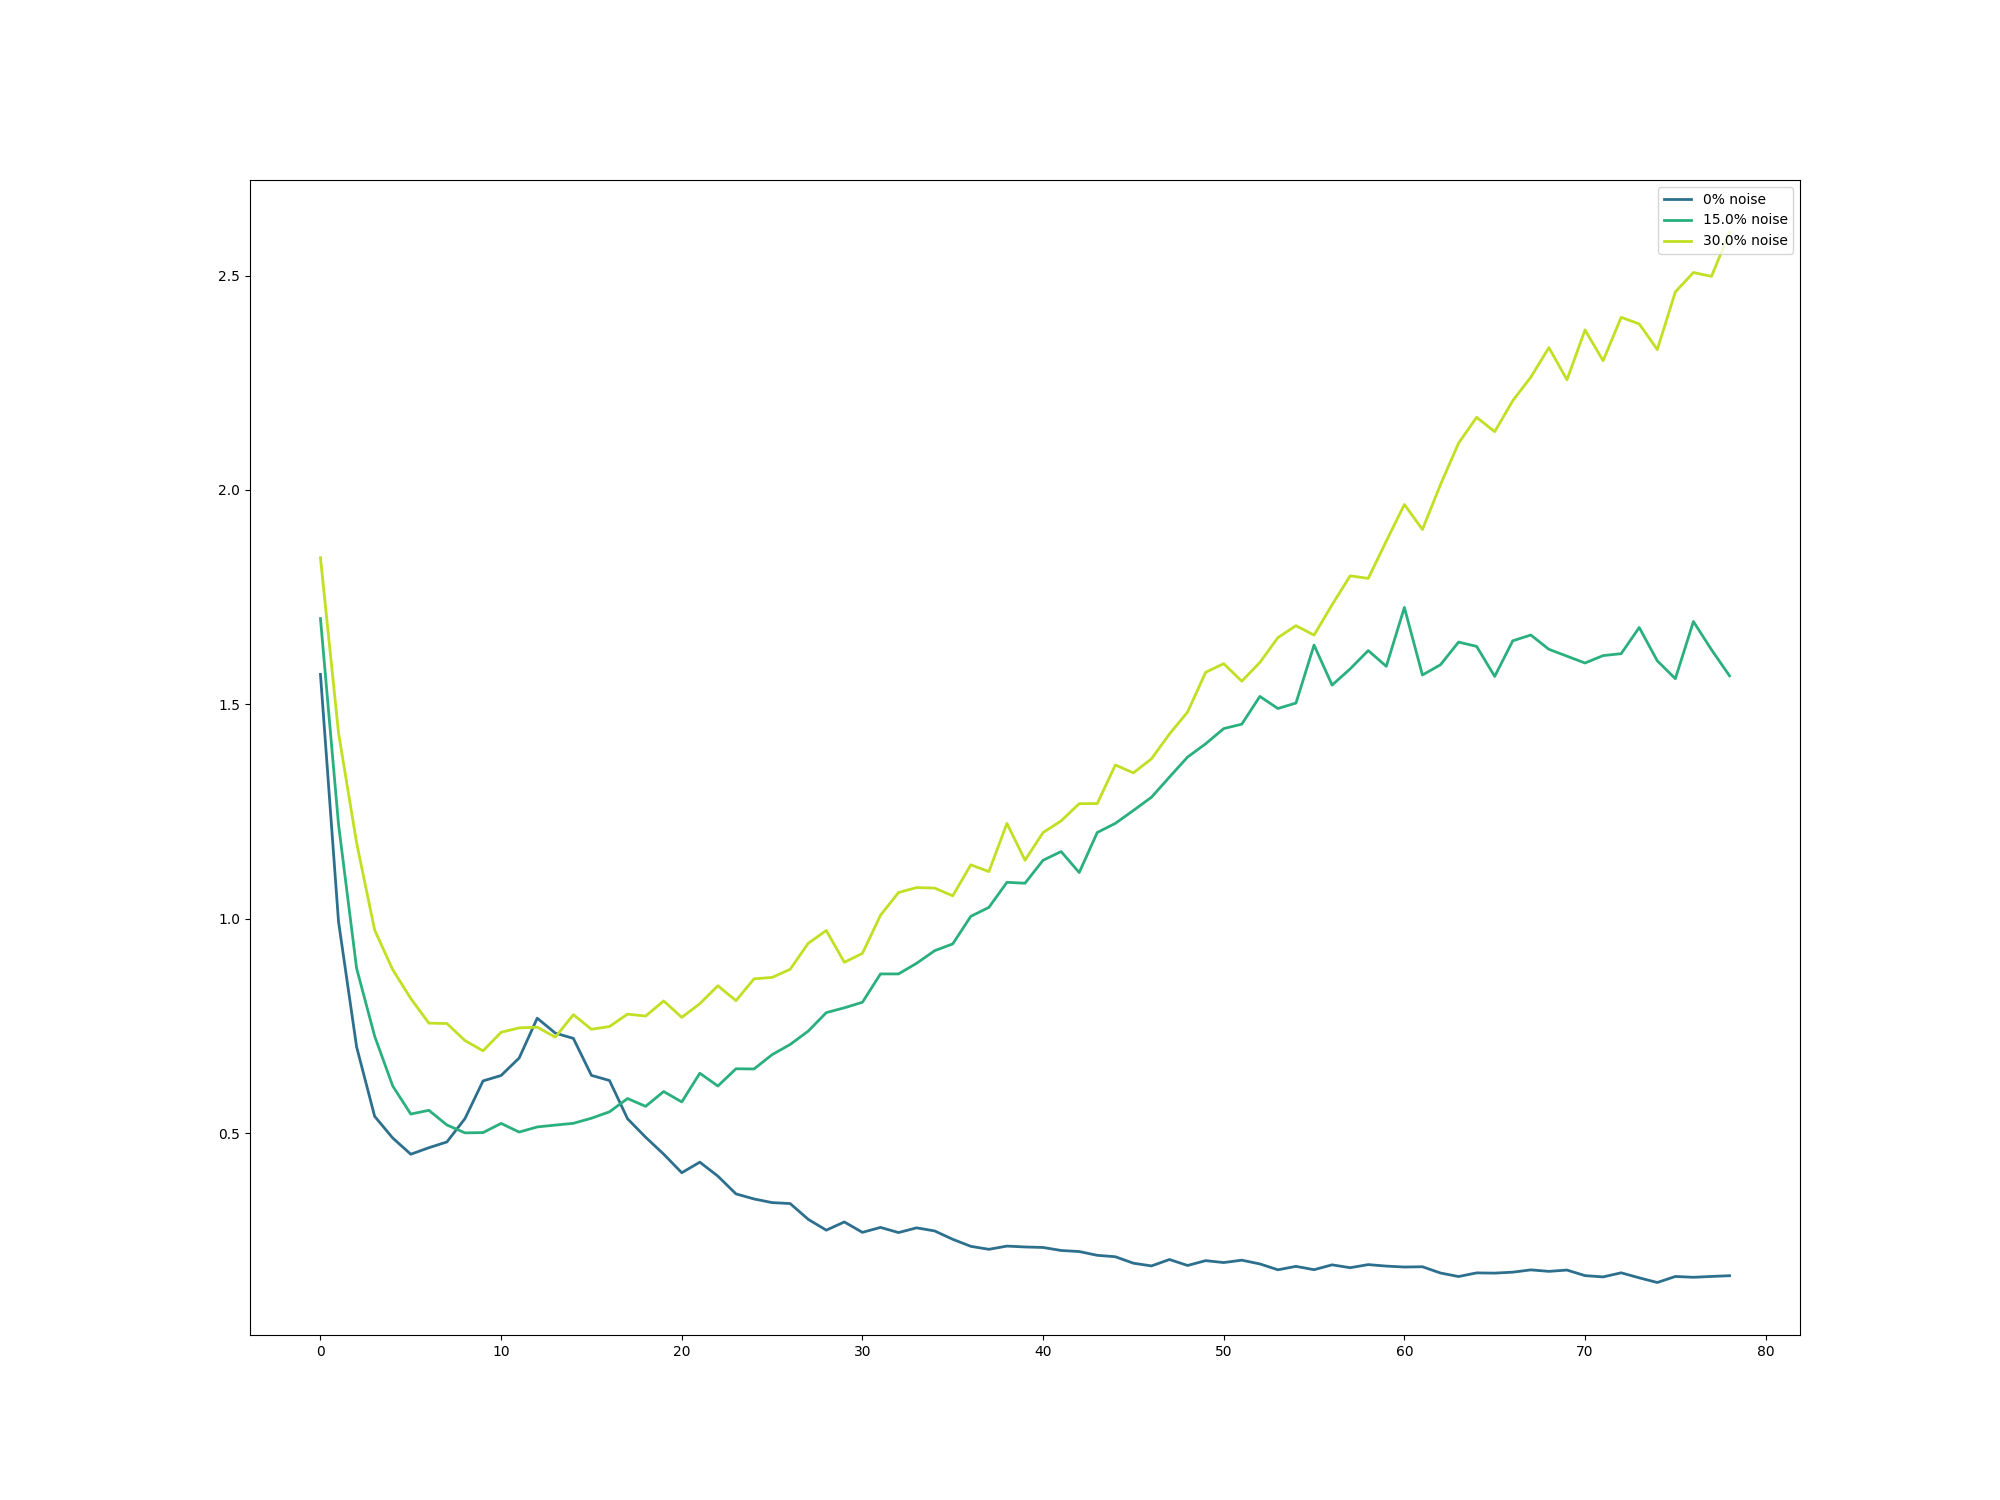
\includegraphics[width= 0.8\linewidth]{Abschlussarbeit_2021/LaTeX/images/noisy_curve.png}
\caption{this graph shows what happens when the noise level is set extremely high. It can be guessed that Double Descent occurs anyway, even if the interpolation threshold occurs only at large layer size $H$. This graph is a supplement to figure \ref{fig:Label_noise_on_double_descent}.}
\label{more_noise_can_hurt}
\end{figure}

\begin{figure}[!htp]
\centering
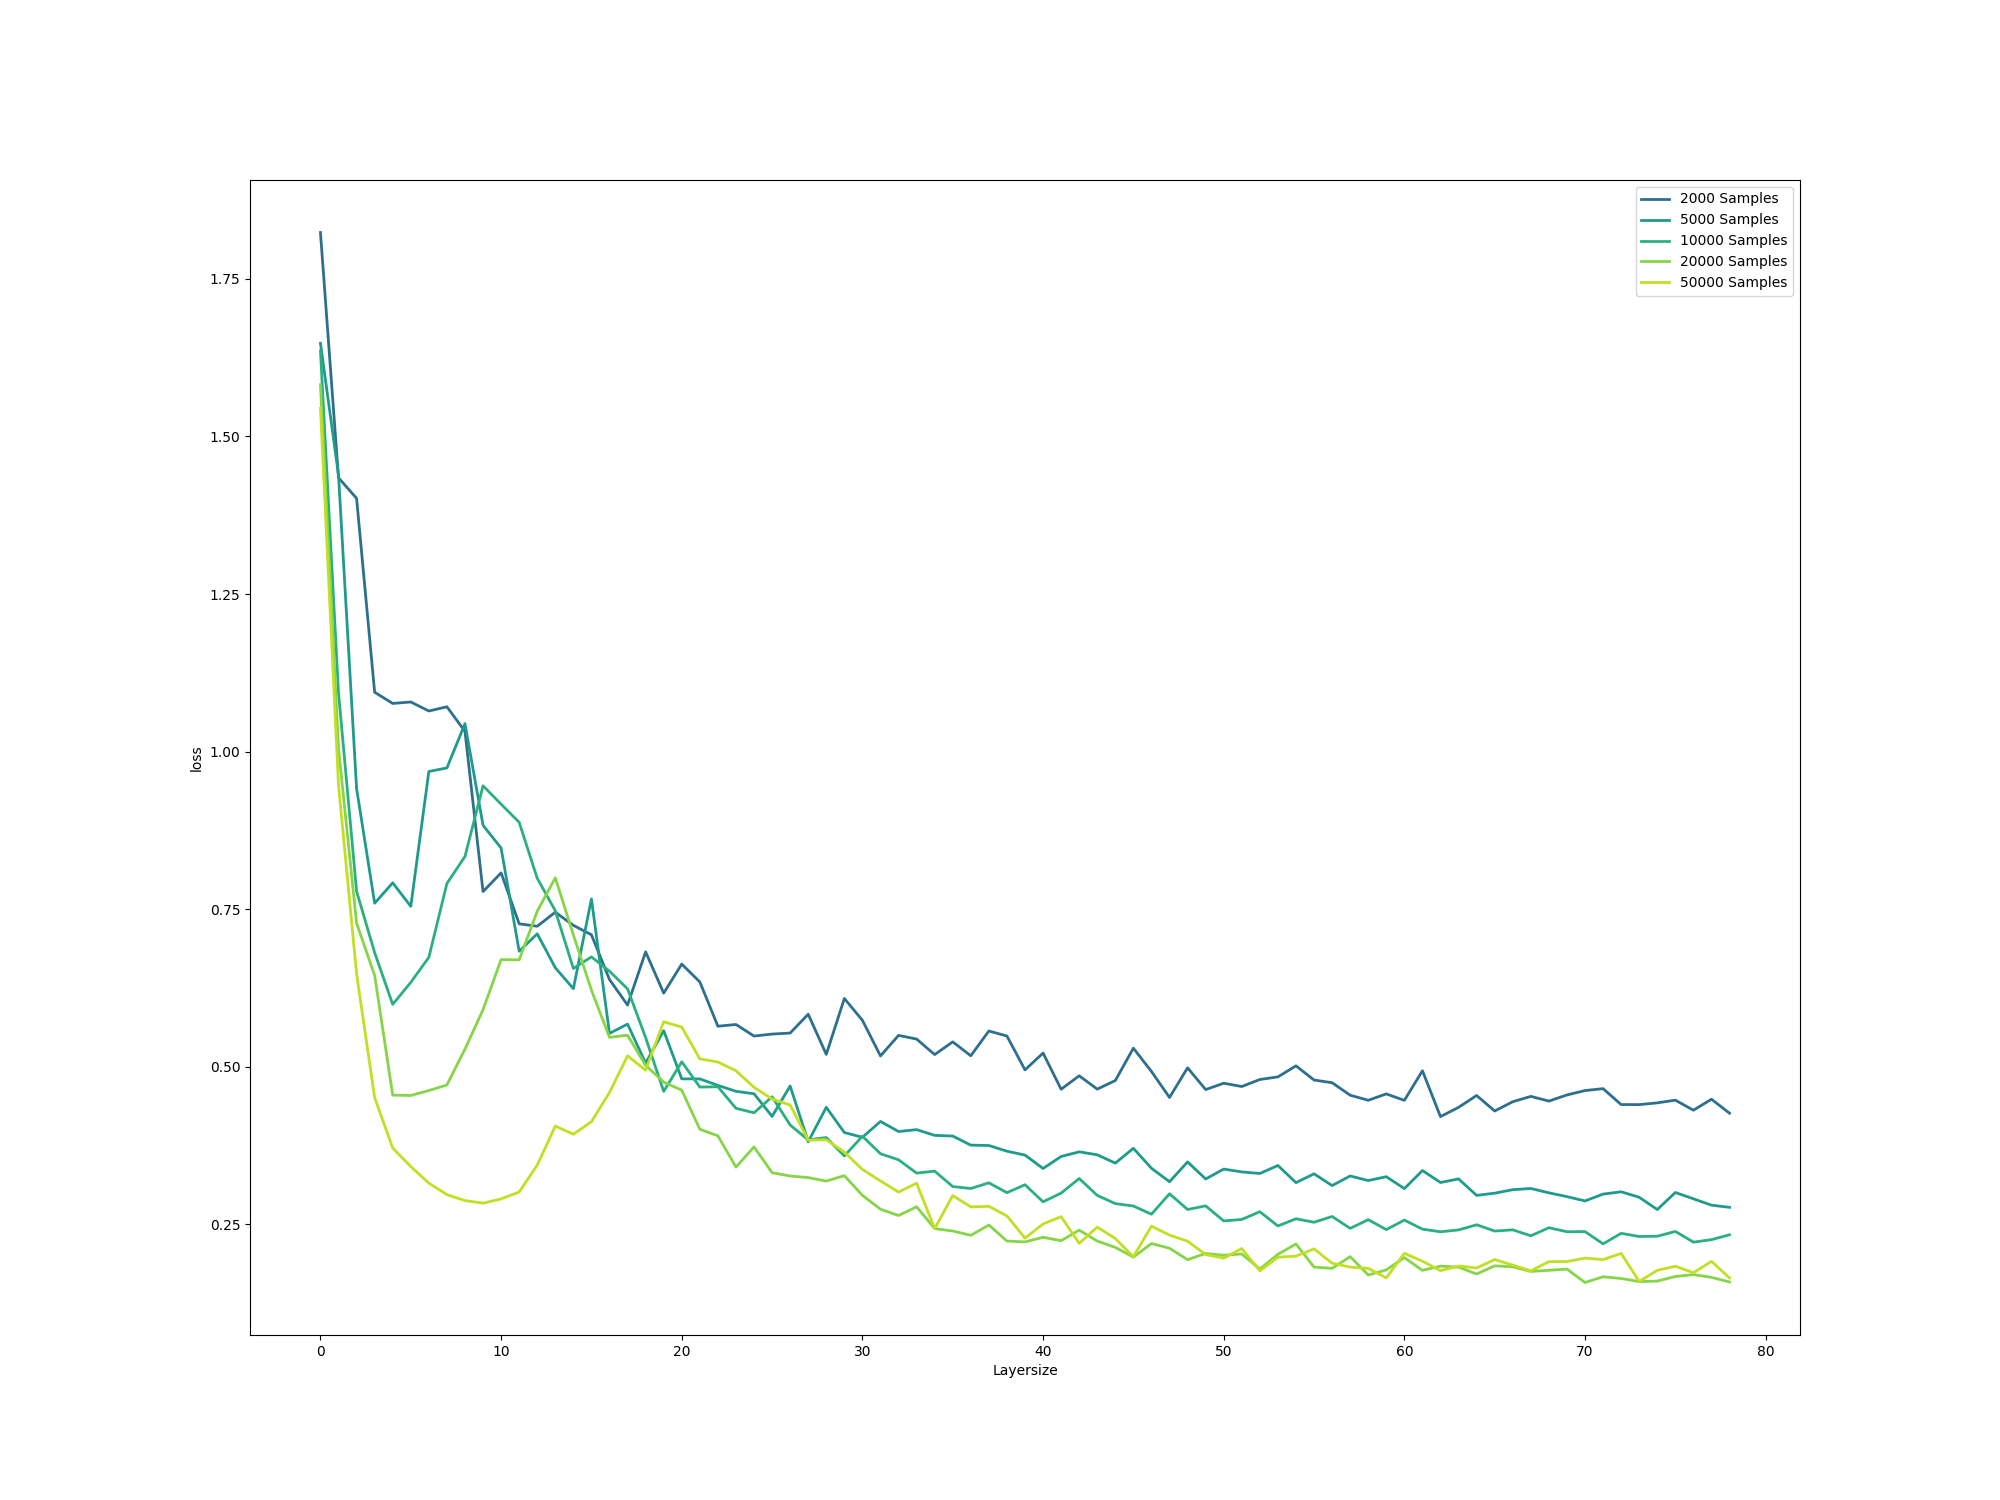
\includegraphics[width= 0.8\linewidth]{Abschlussarbeit_2021/LaTeX/images/many_samplesizes.png}
\caption{This graphic refers to figure \ref{fig:sample_size_double_descent}. Different sample sizes have been added as well. The described effect in \ref{more_noise_can_hurt} can also be observed here.}
\label{more_noise_can_hurt}
\end{figure}


\section{Investigations and possible Explanations for the behavior of the curve}

\subsection{Bias variance trade-off}
\label{bv_help_eq}
We want to show that $E[X^2] = Var[X] + E[X]^2$. \\
This directly follows out of 
$$
Var(X) = E[(X-E[x])^2] = E[X^2] + E[X]^2 - 2E[X\cdot E[x]]
$$
$$
\Longleftrightarrow Var(X) = E[X^2] + E[X]^2 - 2E[X]^2 = E[X^2] - E[X]^2 
$$
$$
\Longleftrightarrow E[X^2] = Var[X] + E[X]^2
$$
This Equation is also known as the displacement theorem from Steiner.

\subsection{Experiments on RFFs}

\subsubsection{Proof for the optimal function in experiment \ref{fig:1d_rff}}
\label{proof_for_1d_rff}
Let $D \in \mathbb{R}^{n \times 2}$ be the generated data points. 
To minimize the Error we have to minimize the term,
$$
\sum_{(x,y) \in D} E[(y - f(x))^2] = \sum_{(x,y) \in D} E[(y)^2] - 2\cdot E[y]\cdot E[f(x)] +  E[f(x)^2]
$$
$$
\Longleftrightarrow \sum_{(x,y) \in D} E[(y - f(x))^2] = \sum_{(x,y) \in D} E[y^2 + f(x)^2] - 2\cdot E[y]\cdot E[f(x)] 
$$
We know that $E[(y - f(x))^2] \geq 0$ and is therefore minimal if $E[(y - f(x))^2] = 0$
$$
\Rightarrow \sum_{(x,y) \in D} E[y^2 + f(x)^2] = \sum_{(x,y) \in D} 2\cdot E[y]\cdot E[f(x)]  
$$
This holds if $E[y] = E[f(x)]$  $\forall (x,y) \in D$. $E[y] = m \cdot x + c$ is given by definition. Therefore,   
$$
f(x) = m\cdot x + c 
$$
is a best possible solution for the problem. And it is also the only global minima because $E[y^2 + f(x)^2] \geq 0$.


\subsubsection{Proof for the optimal function in experiment \ref{3d_RFF}}
Here the same argument as in \ref{proof_for_1d_rff} holds.
Let $D \in \mathbb{R}^{n \times 3}$ be the generated data points. 
To minimize the Error we have to minimize the term,
$$
\sum_{(x,y) \in D} E[(y - f(x))^2] = \sum_{(x,y) \in D} E[(y)^2] - 2\cdot E[y]\cdot E[f(x)] +  E[f(x)^2]
$$
We again use that $E[(y - f(x))^2] \geq 0$ and is therefore minimal if $E[(y - f(x))^2] = 0$
$$
\Rightarrow \sum_{(x,y) \in D} E[y^2] + E[f(x)^2] = \sum_{(x,y) \in D} 2\cdot E[y]\cdot E[f(x)]  
$$
$E[y] = 0$ $\forall (x,y) \in D$ is given by definition. 
$$
\Longleftrightarrow \sum_{(x,y) \in D} E[f(x)^2] = 0
$$
Because $f(x)^2 \geq 0$. The only best possible solution is given by the $x$-$y$-plane,
$$
f(x) = 0 
$$



\newpage

\subsubsection{Extrapolation in the experiment \ref{3d_RFF}}
\label{extrapolation}

It can be observed that models with more parameters perform better even with extrapolation. The successful extrapolation can also be due to the periodic properties of the fourier features.


\begin{figure}[!htp]
\centering
\begin{subfigure}{}
  \centering
  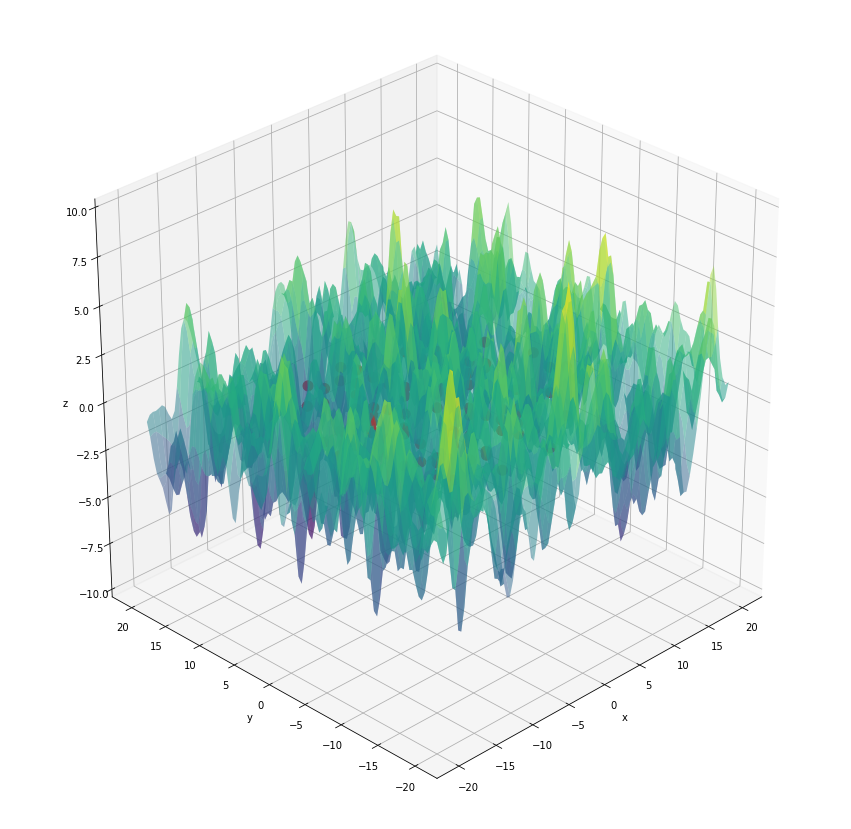
\includegraphics[width=.49\linewidth]{Abschlussarbeit_2021/LaTeX/images/extrapol_less.png}
  \label{fig:sub1}
\end{subfigure}%
\begin{subfigure}{}
  \centering
  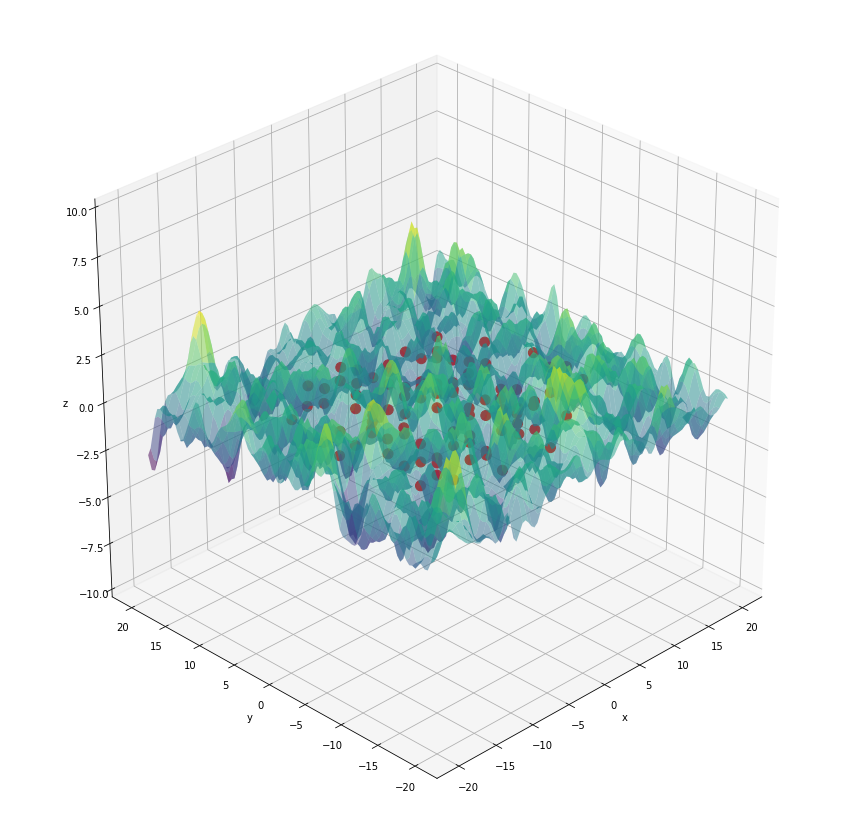
\includegraphics[width=.49\linewidth]{Abschlussarbeit_2021/LaTeX/images/extrapol_many.png}
  \label{fig:sub2}
\label{fig:high_varianz_with_noise}  
\end{subfigure}
\caption{The left plot shows a function learned from a model with $N = 120$ random fourier features. The right plot shows the function learned by a model with $N = 10000$ features. The red points are the data-points. The definition range in which the function is to be predicted is in this example larger as in \ref{3d_RFF} $([-20,20] \times [-20,20])$.}
\label{3d_RFF_extra}
\end{figure}

\subsection{Other interesting discoveries }

\subsubsection{Further plots to the SAM-optimizer }
\label{sam_extension}

In this section it can be observed what happens when the factor $\rho$ is increased in the SAM-optimizer. As mentioned in \ref{fig:sam} the test loss decreases at the interpolation threshold.

\begin{figure}[!htp]
\centering
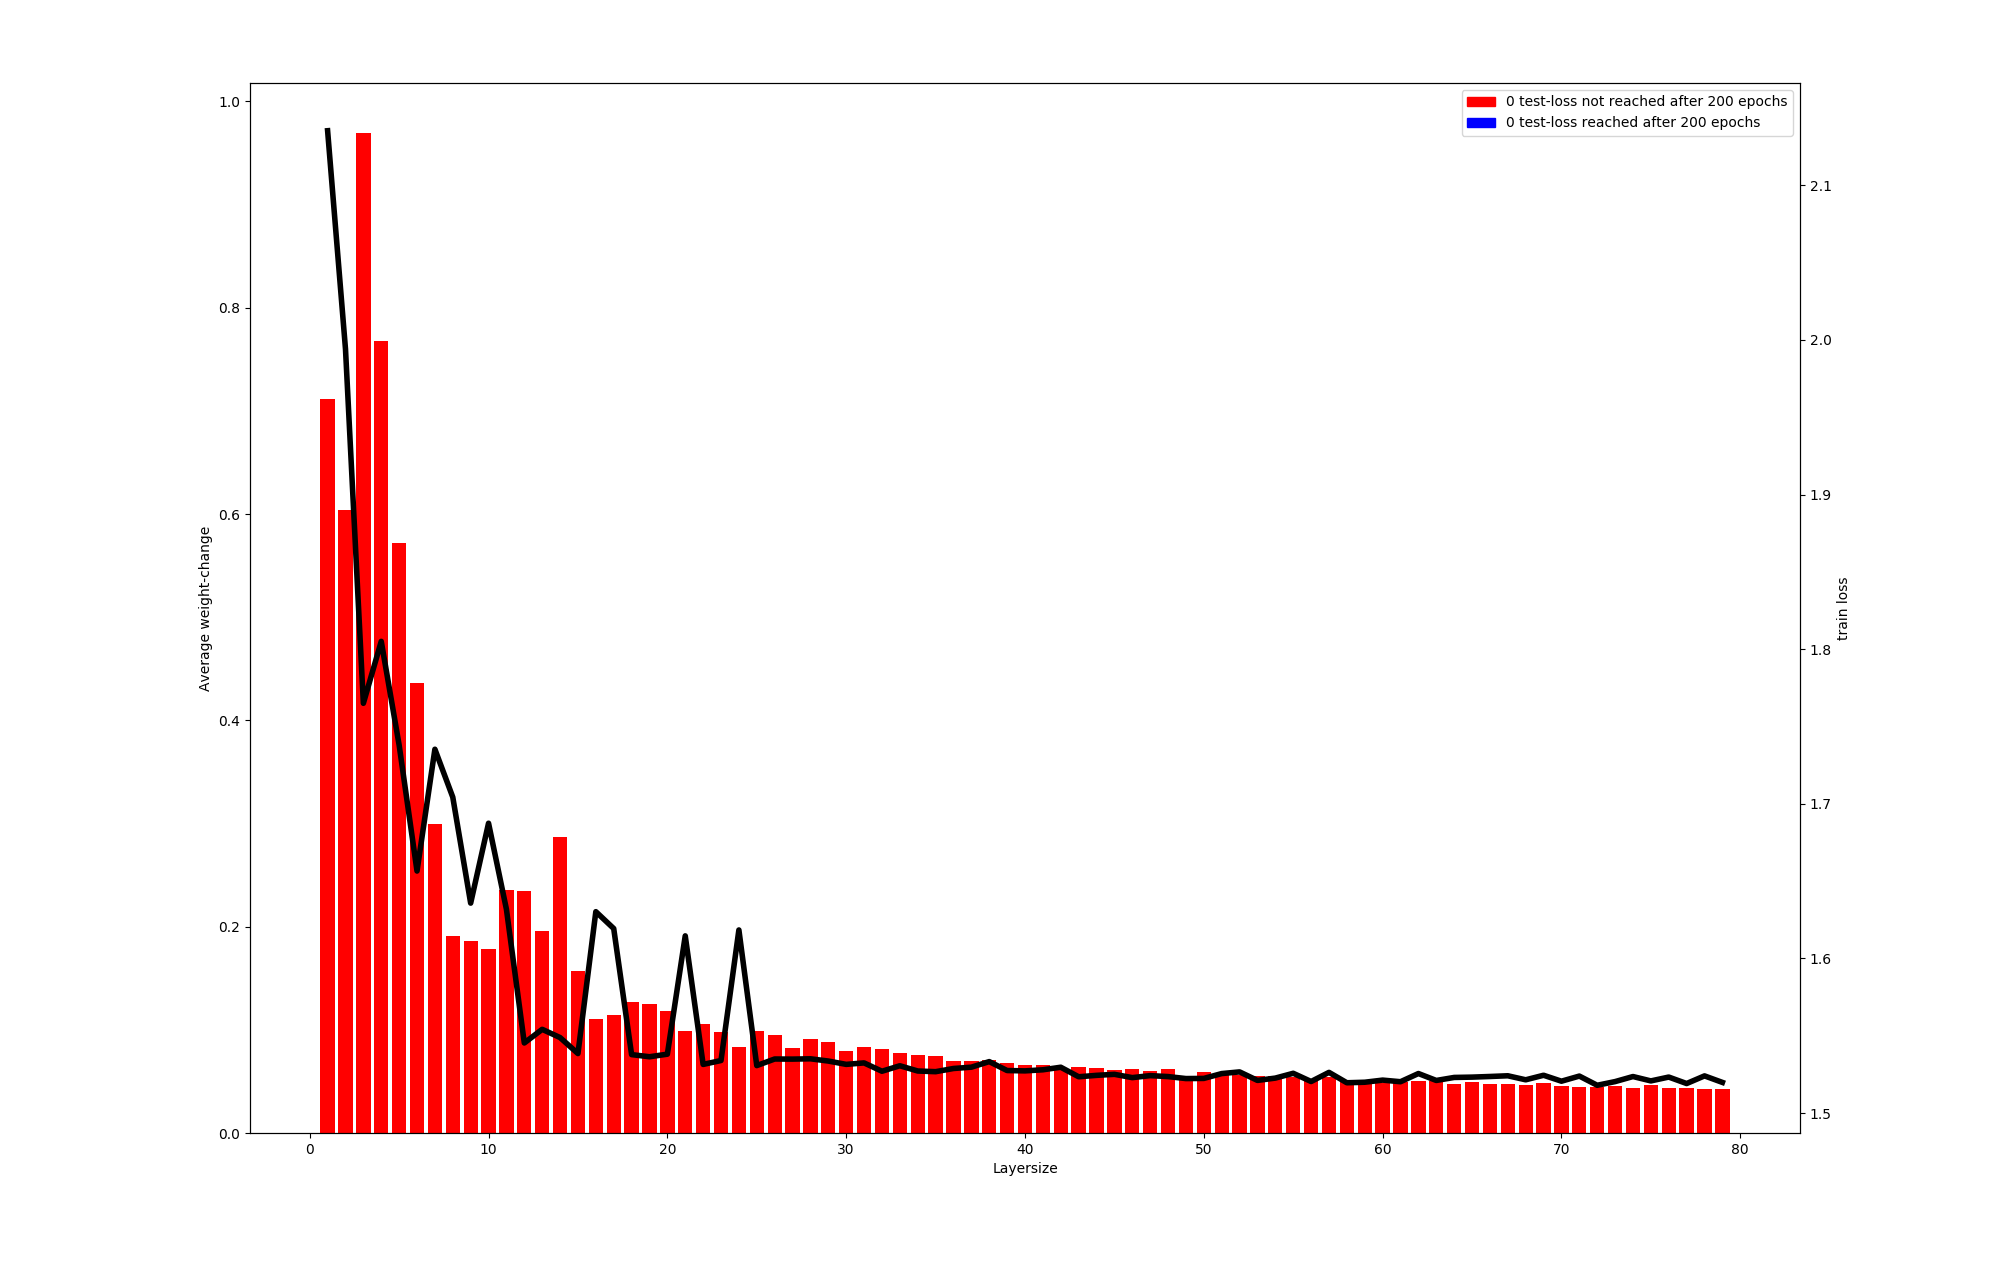
\includegraphics[width= 0.8\linewidth]{Abschlussarbeit_2021/LaTeX/images/sam_weigthchange.png}
\caption{A smoothing factor of $\rho = 0.1$
was used. The data set is a subset of MNIST with 15000 samples}
\label{more_noise_can_hurt}
\end{figure}

\begin{figure}[!htp]
\centering
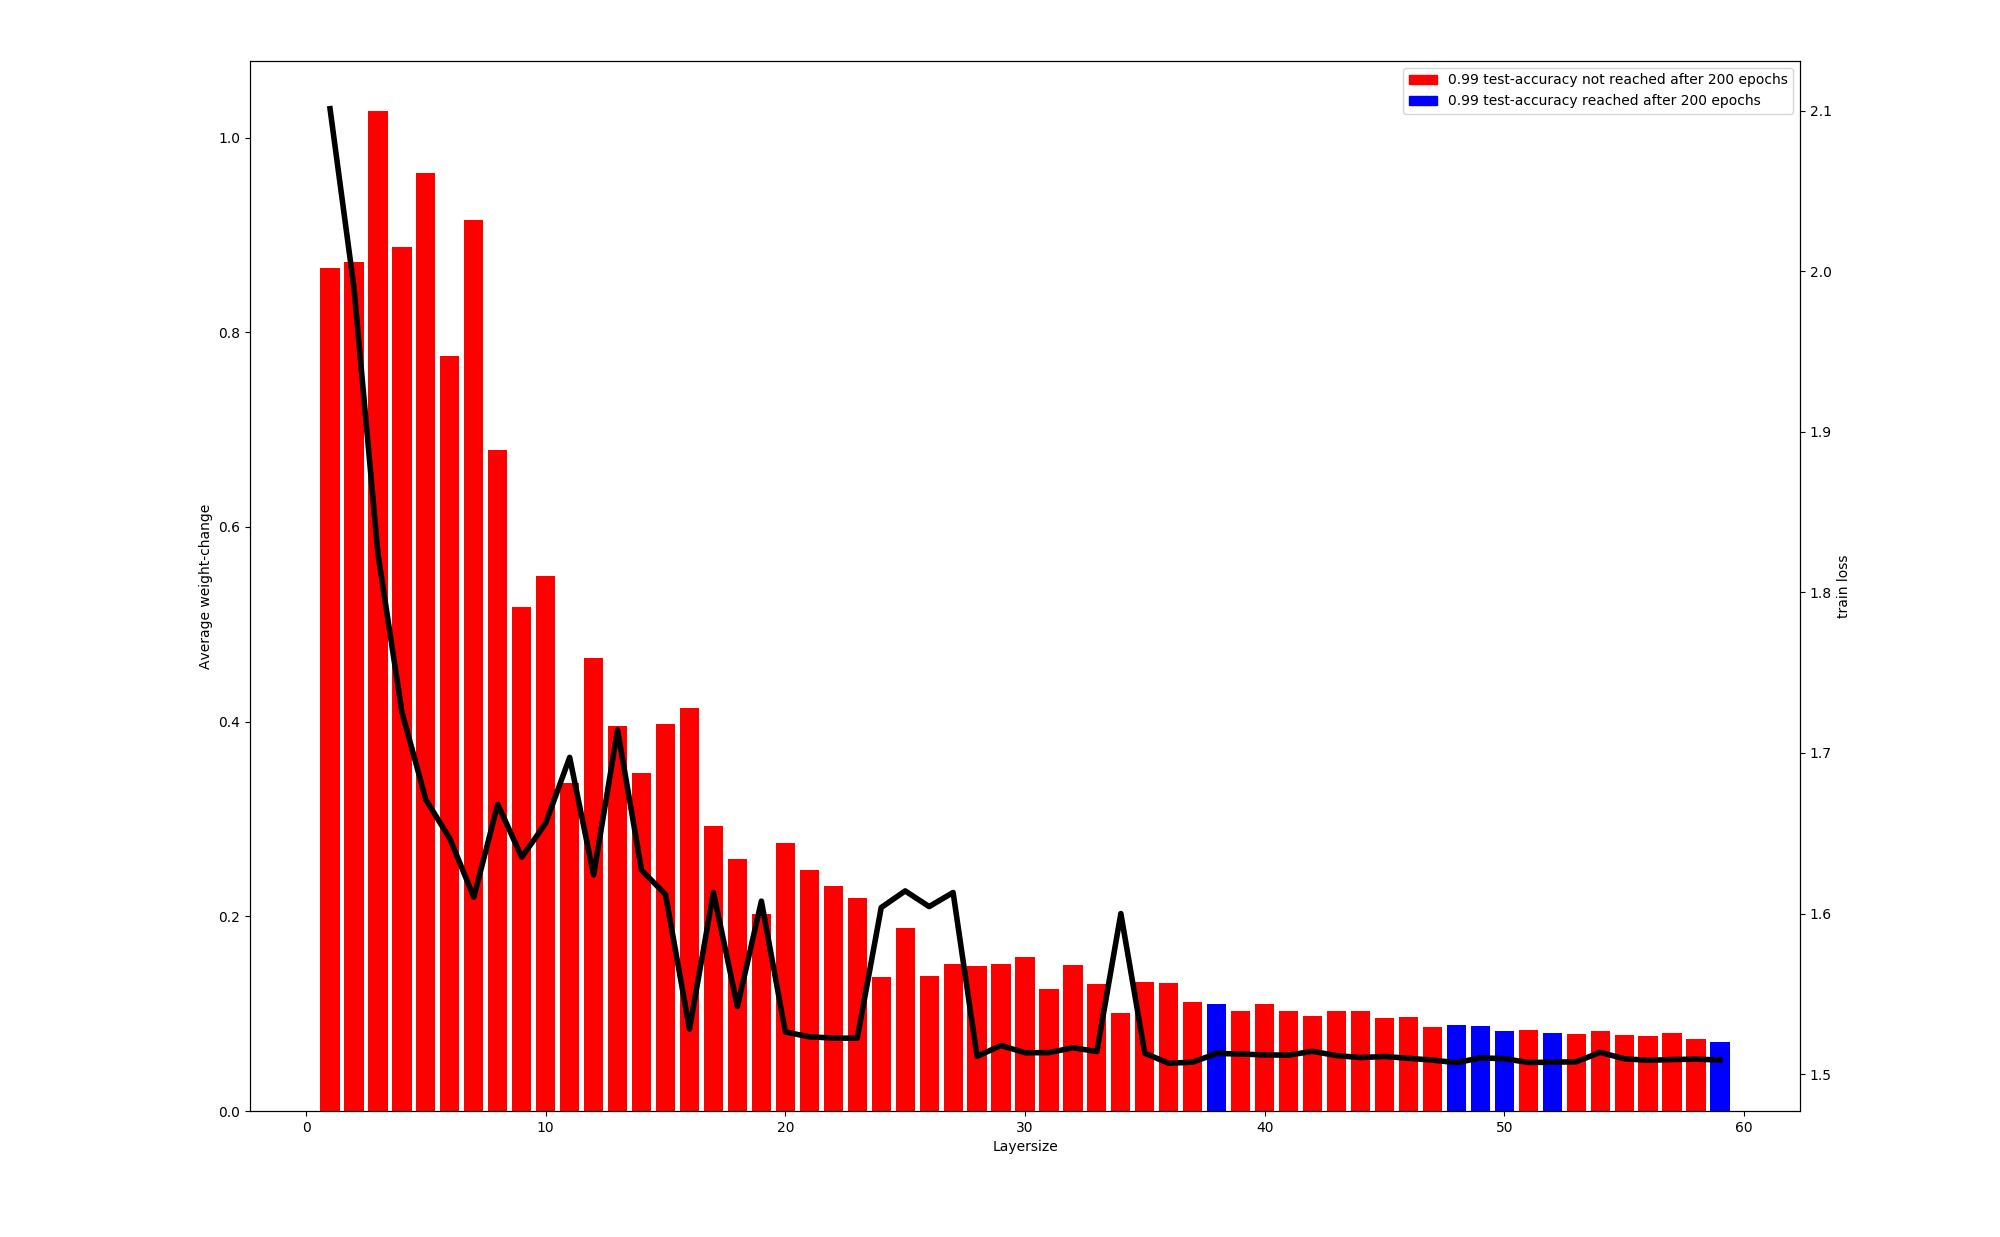
\includegraphics[width= 0.8\linewidth]{Abschlussarbeit_2021/LaTeX/images/sam_loss4_.png}
\caption{A smoothing factor of $\rho = 0.07$
was used. The data set is a subset of MNIST with 15000 samples}
\label{more_noise_can_hurt}
\end{figure}


















